% $Id: simple_fm_receiver.tex,v 1.2 2005-03-29 05:03:21 arif_endro Exp $
%%%%%%%%%%%%%%%%%%%%%%%%%%%%%%%%%%%%%%%%%%%%%%%%%%%%%%%%%%%%%%%%%%%%%%%%
%   Title      : Simple FM Receiver DOCS
%   Project    : FM Receiver
%
%   Author     : Arif E. Nugroho
%
%%%%%%%%%%%%%%%%%%%%%%%%%%%%%%%%%%%%%%%%%%%%%%%%%%%%%%%%%%%%%%%%%%%%%%%%
%  Description : Simple FM Receiver documentations file
%
%  Copyright (c) 2005 Arif E. Nugroho
%%%%%%%%%%%%%%%%%%%%%%%%%%%%%%%%%%%%%%%%%%%%%%%%%%%%%%%%%%%%%%%%%%%%%%%%

\documentclass[a4paper,10pt]{article}

\usepackage[english]{babel}  % enable selecting language in docs
\usepackage{fancybox}        % enable custom box
\usepackage{fancyhdr}        % enable custom header
\usepackage{float}           % enable floating graphics
\usepackage{graphicx}        % enable graphics in docs
\usepackage{palatino}        % palatino font
\usepackage{indentfirst}     % first indentation after section

\setlength{\parindent}        {1cm}
\setlength{\topmargin}        {0cm}
\setlength{\headheight}       {1cm}
\setlength{\textheight}       {21cm}
\setlength{\textwidth}        {16cm}
\setlength{\oddsidemargin}    {0cm}
\setlength{\evensidemargin}   {0cm}
\setlength{\columnsep}        {0.125in}
\setlength{\columnseprule}    {0.5pt}
\setlength{\footskip}         {1cm}
\renewcommand{\footrulewidth} {0.4pt}

% fancy box package 

\newlength{\verbatimbox}
\settowidth{\verbatimbox}{\scriptsize\tt
xxxxxxxxxxxxxxxxxxxxxxxxxxxxxxxxxxxxxxxxxxxxxxxxxxxxxxxxxxxxxxxxxxxxxxxxxxxxxxxx
}

\newenvironment{sourcelisting}
   {\VerbatimEnvironment\par\noindent\scriptsize
    \begin{Sbox}\begin{minipage}{\verbatimbox}\begin{Verbatim}}%
   {\end{Verbatim}\end{minipage}\end{Sbox}
    \setlength{\fboxsep}{3mm}\center
    \shadowbox{\TheSbox}\normalsize\par\noindent}

\newenvironment{commandline}
   {\VerbatimEnvironment\par\vspace*{2mm}\noindent\footnotesize
    \begin{Sbox}\begin{minipage}{\verbatimbox}\begin{Verbatim}}%
   {\end{Verbatim}\end{minipage}\end{Sbox}\setlength{\shadowsize}{2pt}%
    \shadowbox{\TheSbox}\normalsize\par\noindent}

% custom numbering system

\makeatletter

\renewcommand\theequation{\arabic{section}-\arabic{equation}}
\@addtoreset{equation}{section}

\renewcommand\thefigure{\arabic{section}-\arabic{figure}}
\@addtoreset{figure}{section}

\renewcommand\thetable{\arabic{section}-\arabic{table}}
\@addtoreset{table}{section}

\makeatother

% fancy header package

\chead{}
\lhead{\Large \bfseries \texttt{Simple FM Receiver}}
\rhead{\thepage}
\lfoot{\bfseries \texttt{Arif E. Nugroho}}
\cfoot{www.opencores.org}
\rfoot{}

\begin{document}

% Cover

\begin{titlepage}
\thispagestyle{empty}

\begin{center}

\Huge \textbf {\textit{Simple FM Receiver}}

\vspace{3.0cm}
\large \textbf {\texttt{Arif E. Nugroho \\<arif\_endro@opencores.org>}}

\end{center}

\vspace{3.0cm}
\begin{figure}[H]
\center
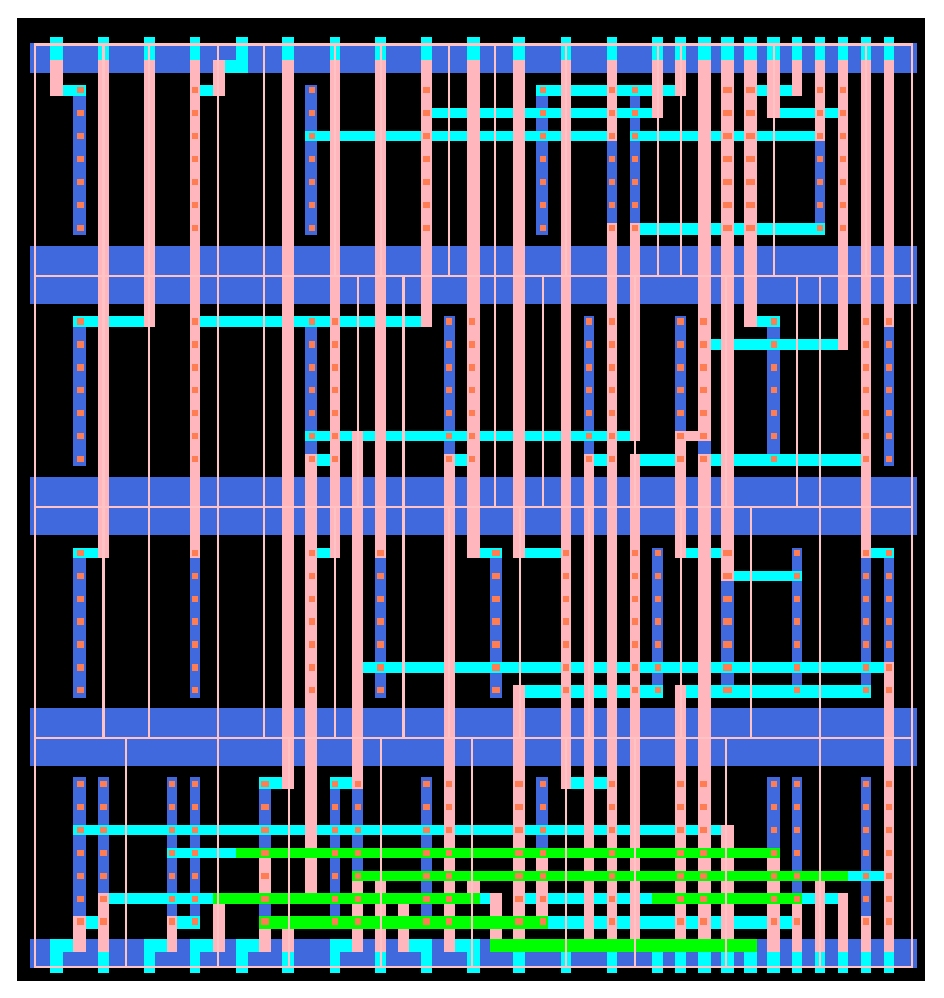
\includegraphics[width=7.5cm,height=7.5cm]{fm_cores.eps}
\end{figure}

\vspace{0.50cm}
\begin{tabular}{p{3.0cm}p{10cm}}
		& VLSI Research Group ITB\\
		& LabTek VIII Institut Teknologi Bandung\\
		& Jl. Ganesha 10 Bandung 40141 West Java Indonesia\\
\end{tabular}

\vspace{1.00cm}
\begin{center}

\Large \textbf{\texttt{2005}}

\end{center}

\end{titlepage}

\pagenumbering{roman}
\tableofcontents
\newpage

\listoffigures
\newpage

\section{Introduction}

\pagestyle{fancy}
\pagenumbering{arabic}

This design is a very simple implementation of FM Receiver for
demodulating Frequency Modulated (FM) signal.  The input signal it's
self is a square wave signal that already modulated and digitized in the
form 8 bit signed 2's complement.

\subsection{Circuit Schematics}

The works of this FM Receiver is based on PLL operation to capture FM
signal.  The design architecture it's self like ordinary PLL using phase
detector, vco (realize using an nco), loop filter, and low pass filter.

\begin{figure}[H]
\center
\includegraphics[width=15cm,height=12cm]{fm_receiver.eps}
\caption {Architecture Schematics}
\end{figure}

In the PLL loop's, the FM signal it's self captured from phase
difference betwee input signal and loop signal. This signal is raw
signal of the original signal and the looks is not too good, After loop
filtering the phase difference looks more clearly. finally, after
filtering out in low pass filter the original signal can be recovered.

The recovered signal it's self not perfect but it's not too far from
original signal. The shape of original signal suppose to be straigh line
but the recovered signal not. There is still many noise in the recovered
signal.

\section{Circuit Component}

\subsection{Core Component}

\begin{itemize}

\item \textbf{fm}

The core component, the connector between many component in the PLL
loops.

\begin{figure}[H]
\center
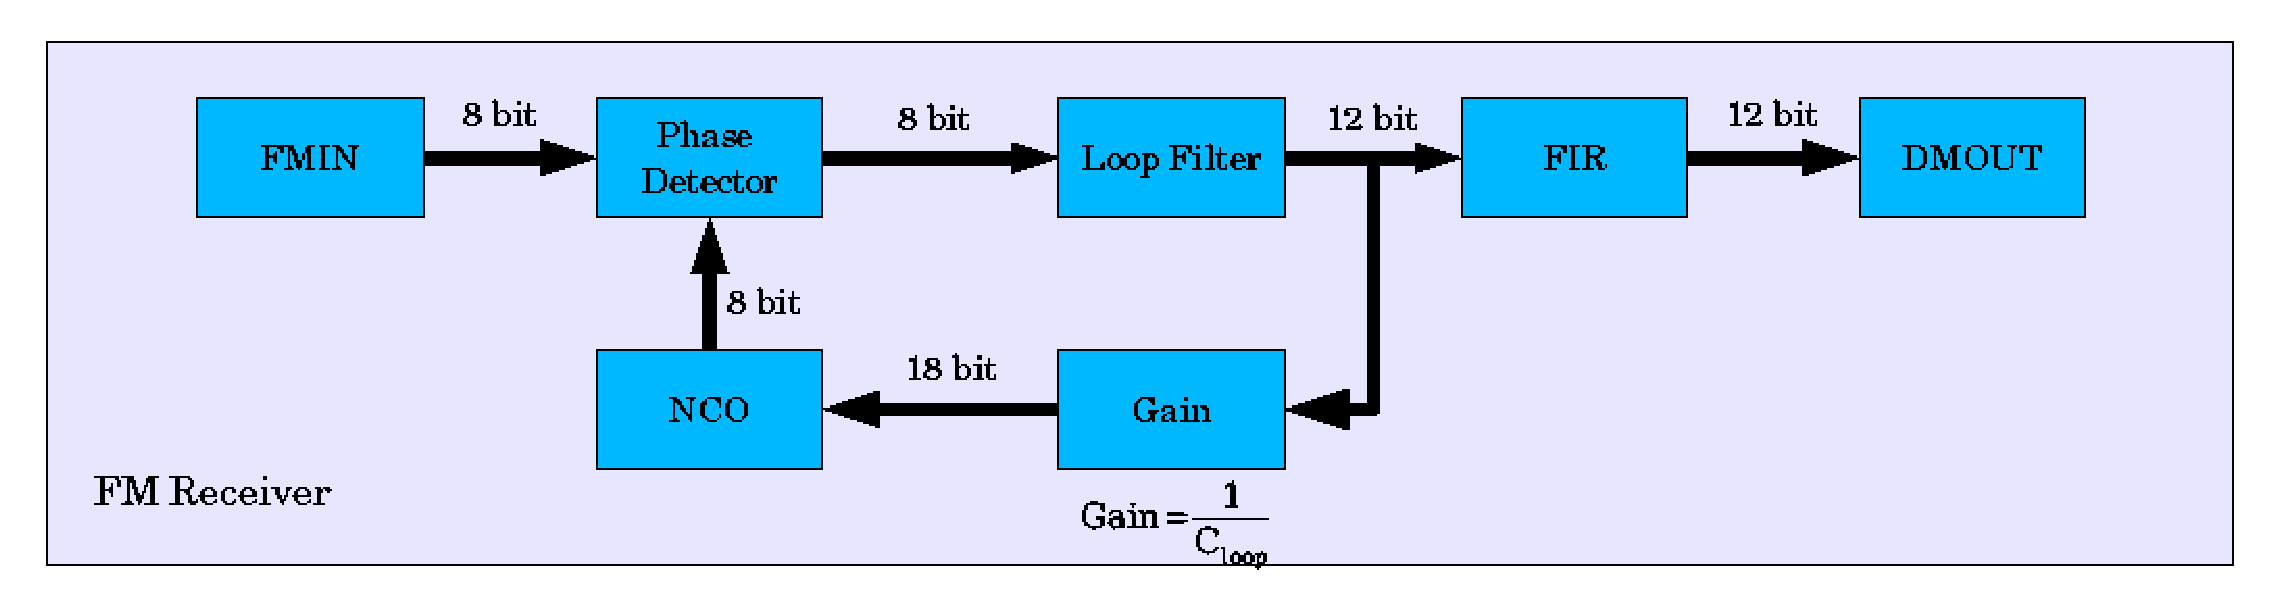
\includegraphics[width=10.0cm,height=5.0cm]{fm.eps}
\caption {FM core component}
\end{figure}

\end{itemize}

\subsection{Main Component}

\begin{itemize}

\item \textbf{nco}

The NCO functions it's like VCO in analog PLL. 

% This NCO works like variable binary up-counter that controlled by input.
% Because its controlled by input then it's output frequency is change
% along with it's input value.

\begin{figure}[H]
\center
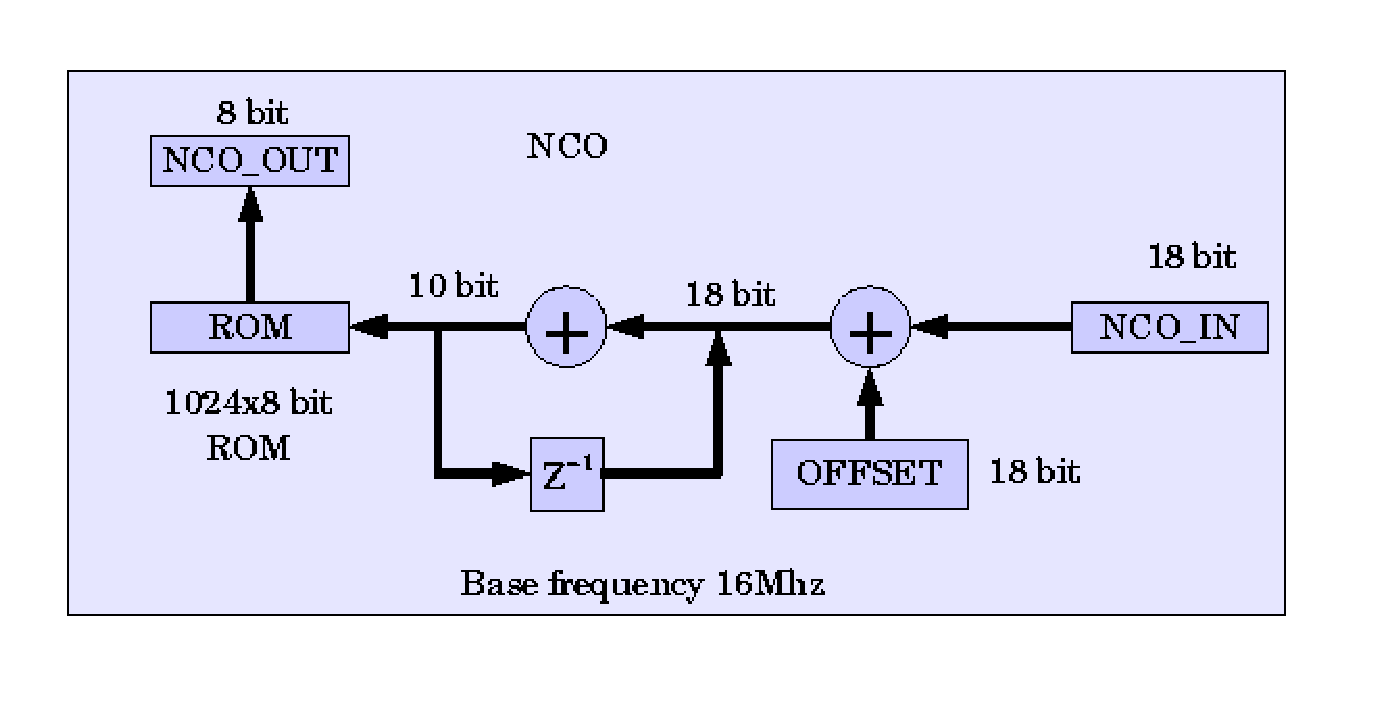
\includegraphics[width=10.0cm,height=5.0cm]{nco.eps}
\caption {NCO block diagram}
\end{figure}

\item \textbf{phase\_detector}

This component works by multiplying input signal
and loop signal.

\begin{figure}[H]
\center
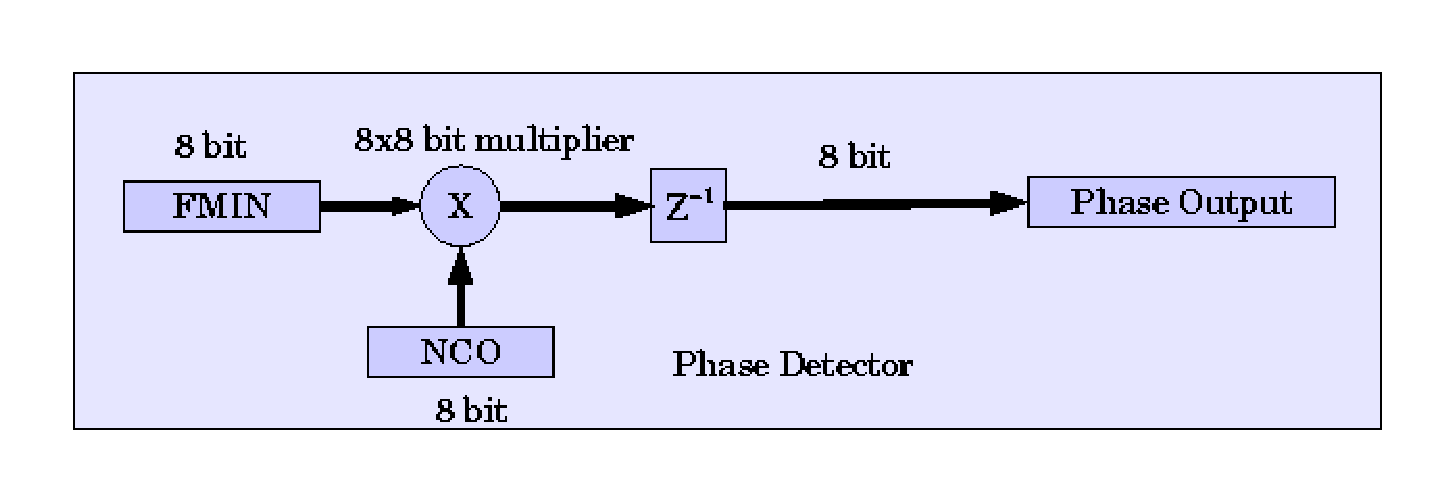
\includegraphics[width=10.0cm,height=5.0cm]{phase_detector.eps}
\caption {Phase detector block diagram}
\end{figure}

\item \textbf{loop\_filter}

A low pass filter in the PLL loop.

%\begin{displaymath}
%Y(z) = X(z) \frac{z^{-1}}{1-(1-\frac{1}{16})z^{-1}}
%\end{displaymath}

\begin{figure}[H]
\center
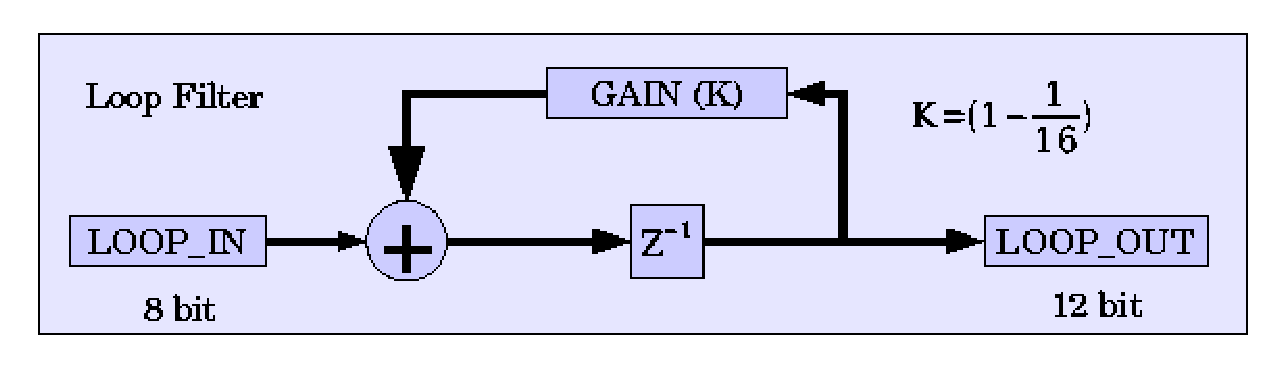
\includegraphics[width=10.0cm,height=5.0cm]{loop_filter.eps}
\caption {Loop filter block diagram}
\end{figure}

% \item \textbf{low pass filter}
% 
% Realization of this filter is using direct FIR Transform 16 tap.
% 
% \begin{displaymath}
% Y(z) = X(z) \frac{1}{C_{fir}}\sum_{i=0}^{15}z^{-i}
% \end{displaymath}

\end{itemize}

\subsection{Arithmetic Component}

\begin{itemize}

\item \textbf{adder}

Adder implementation in this design is in the simplest form (e.g simple
ripple carry adder), this adder implementations is the slowest compared
with other type adder but this adder implementations is easy to
understand. This adder is used for arithmetics operations in many
component that exists in the PLL loops\footnote{I will use a different
type adder for next time, if you have any suggestion email me :)}.

\item \textbf{subtractor}

Subtractor implementation used in this design is a modified version of
adder. This is because the subtractor it's self a manipulations of
adder\footnote{in 2's complement implementation negatif value of a
number is equal to it's 2' complement. so subtraction is equal to
addition to it's 2's complement}.

\item \textbf{multiplier}

Multiplier is used on the phase detector to multiply input signal and
signal nco to get the phase different.  

% This multiplier is implemented using simple addition of two operand.
% this multiplier need 8 stage of addition to perform operation on 8 bit
% input operand. This multiplier is the slowest component in this design,
% because this operations takes 8 stages of additions to complete single
% multiplications.
% 
% \begin{sourcelisting}
% operand0          = XXXX_XXXX
% operand1          = XXXX_XXXX
% _____________________________
% ...
% ...       -> 8 stage addition
% ...
% _____________________________
% result = XXXX_XXXX__XXXX_XXXX
%          ^^^^^^^^^--> 8 bit output
% \end{sourcelisting}

\item \textbf{full adder}

Full Adder, everyone already know about it's. In this design the full
adder implementation is implemented using following
relations\footnote{because full adder input/output relations can have
many form, if you have better implementation just let me know :)}:

\begin{sourcelisting}
sum          <=  ((addend xor augend) xor carry_in);
carry        <=  ((addend xor augend) or  (carry_in and (addend or augend)));
\end{sourcelisting}

\end{itemize}

\section{Waveform}

Here is the output waveform of the design.

\begin{figure}[H]
\center
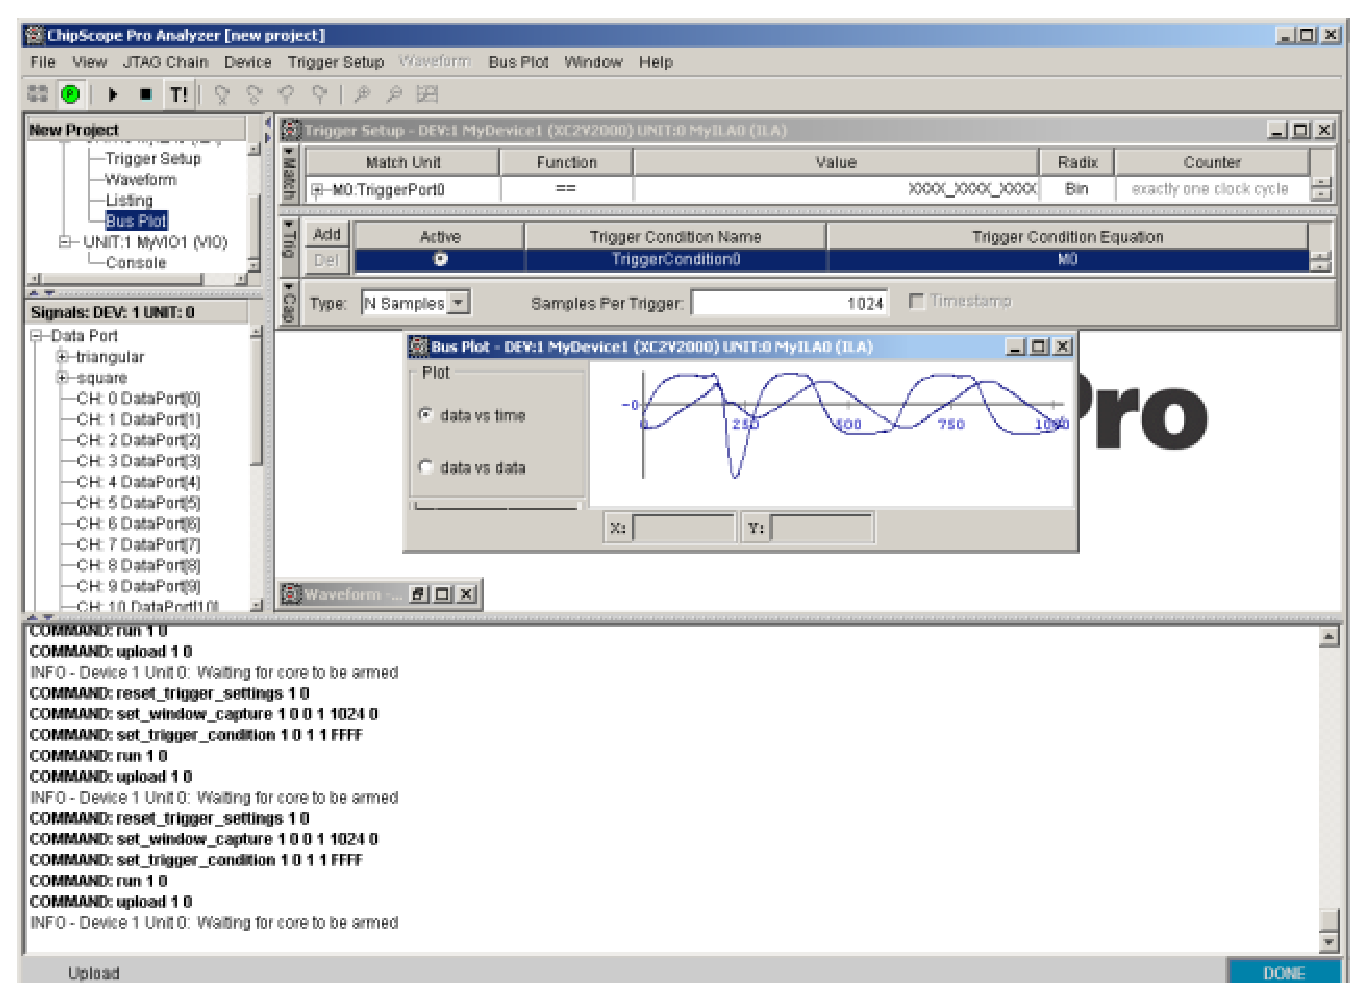
\includegraphics[width=15cm,height=10cm]{screenshot.eps}
\caption {Waveform preview}
\end{figure}

\newpage

\section{Information}

\subsection{Warranty}

\begin{center}
		\textbf	     {\texttt{NO WARRANTY}}\\
\end{center}

\scriptsize
\textbf{\textrm{
THIS SOFTWARE IS PROVIDED BY THE AUTHOR ``AS IS'' AND ANY EXPRESS OR
IMPLIED WARRANTIES, INCLUDING, BUT NOT LIMITED TO, THE IMPLIED WARRANTIES
OF MERCHANTABILITY AND FITNESS FOR A PARTICULAR PURPOSE ARE DISCLAIMED.
IN NO EVENT SHALL THE AUTHOR BE LIABLE FOR ANY DIRECT, INDIRECT,
INCIDENTAL, SPECIAL, EXEMPLARY, OR CONSEQUENTIAL DAMAGES (INCLUDING, BUT
NOT LIMITED TO, PROCUREMENT OF SUBSTITUTE GOODS OR SERVICES; LOSS OF USE,
DATA, OR PROFITS; OR BUSINESS INTERRUPTION) HOWEVER CAUSED AND ON ANY
THEORY OF LIABILITY, WHETHER IN CONTRACT, STRICT LIABILITY, OR TORT
(INCLUDING NEGLIGENCE OR OTHERWISE) ARISING IN ANY WAY OUT OF THE USE OF
THIS SOFTWARE, EVEN IF ADVISED OF THE POSSIBILITY OF SUCH DAMAGE.
}}
\normalsize

\subsection{TOOLS}

\begin{itemize}

\item \textbf{\texttt{ALLIANCE CAD SYSTEM}} developed by \textbf{\texttt{ASIM}}
      team at \copyright \textbf{\texttt{LIP6}}/Universit\'{e} Pierre et
      Marie Curie,
      \texttt{http://asim.lip6.fr/recherche/alliance} 
      - \textbf{\textit{The primary VHDL Analyser for Synthesize}}

\item \textbf{\texttt{ISE Xilinx 6.3i}} - \textbf{\textit{The Synthesizer}}

\item \textbf{\texttt{VIM - Vi IMproved}}
      - \textbf{\textit{The Editor}}

\item \LaTeX - \textbf{\textit{The Typesetter}}

\end{itemize}

\begin{thebibliography}{1}

\bibitem{Wada} Tom Wada,
	\textbf{\textit{ All Digital FM Receiver}}, at
	http://www.ie.u-ryukyu.ac.jp/\~\ wada/design05/

\end{thebibliography}

\vspace{01cm}

\begin{tabbing}
\textbf{Version: 1.2}  \` \textbf{\today}
\end{tabbing}

\end{document}
